%%%%%%%%%%%%%%%%%%%%%%%%%%%%%%%%%%%%%%%%%
% Beamer Presentation
% LaTeX Template
% Version 1.0 (10/11/12)
%
% This template has been downloaded from:
% http://www.LaTeXTemplates.com
%
% License:
% CC BY-NC-SA 3.0 (http://creativecommons.org/licenses/by-nc-sa/3.0/)
%
%%%%%%%%%%%%%%%%%%%%%%%%%%%%%%%%%%%%%%%%%

%----------------------------------------------------------------------------------------
%	PACKAGES AND THEMES
%----------------------------------------------------------------------------------------

\RequirePackage{currfile} 


\documentclass{beamer}


\mode<presentation> {

% The Beamer class comes with a number of default slide themes
% which change the colors and layouts of slides. Below this is a list
% of all the themes, uncomment each in turn to see what they look like.

%\usetheme{default}
%\usetheme{AnnArbor}
%\usetheme{Antibes}
%\usetheme{Bergen}
%\usetheme{Berkeley}
%\usetheme{Berlin}
%\usetheme{Boadilla}
%\usetheme{CambridgeUS}
%\usetheme{Copenhagen}
%\usetheme{Darmstadt}
%\usetheme{Dresden}
%\usetheme{Frankfurt}
%\usetheme{Goettingen}
%\usetheme{Hannover}
%\usetheme{Ilmenau}
%\usetheme{JuanLesPins}
%\usetheme{Luebeck}
%\usetheme{Madrid}		
%\usetheme{Malmoe}
%\usetheme{Marburg}
%\usetheme{Montpellier}
%\usetheme{PaloAlto}
%\usetheme{Pittsburgh}
%\usetheme{Rochester}
%\usetheme{Singapore}
%\usetheme{Szeged}
\usetheme{Warsaw}

% As well as themes, the Beamer class has a number of color themes
% for any slide theme. Uncomment each of these in turn to see how it
% changes the colors of your current slide theme.

%\usecolortheme{albatross}
%\usecolortheme{beaver}
%\usecolortheme{beetle}
%\usecolortheme{crane}
%\usecolortheme{dolphin}
%\usecolortheme{dove}
%\usecolortheme{fly}
%\usecolortheme{lily}
%\usecolortheme{orchid}
%\usecolortheme{rose}
%\usecolortheme{seagull}
%\usecolortheme{seahorse}
\usecolortheme{whale}
%\usecolortheme{wolverine}

%\setbeamertemplate{footline} % To remove the footer line in all slides uncomment this line
%\setbeamertemplate{footline}[frame number] % To replace the footer line in all slides with a simple slide count uncomment this line

%\setbeamertemplate{navigation symbols}{} % To remove the navigation symbols from the bottom of all slides uncomment this line

\setbeamercovered{transparent} % Fait apparaître les animations en grisé (utile pour la conception, mais peut être commenté lors de la remise du document final)

% Pour utiliser une police à empattements partout
\usefonttheme{serif}

% Pour rajouter la numérotation des frames dans les pieds de page
\newcommand*\oldmacro{}%
\let\oldmacro\insertshorttitle%
\renewcommand*\insertshorttitle{%
  \oldmacro\hfill%
  \insertframenumber\,/\,\inserttotalframenumber}

}

\usepackage{graphicx} % Allows including images
\usepackage{booktabs} % Allows the use of \toprule, \midrule and \bottomrule in tables

\usepackage[utf8]{inputenc}
\usepackage{graphicx}
\usepackage{listings}



\usepackage[utf8]{inputenc}
\begin{document}
QUESTION-Find the equation of the tangent to the circle,
at the point "B"-
$$
\mathsf{B} =
\begin{pmatrix}
1\\
-1
\end{pmatrix}
$$
whose centre is the point of intersection of the
straight lines


\begin{align}
\begin{pmatrix}
    2 & 1 
\end{pmatrix}
\times
\begin{pmatrix}
    x \\
    y
\end{pmatrix}
=
\begin{pmatrix}
    3  \\
\end{pmatrix}
\end{align}


\begin{align}
\begin{pmatrix}
    1 & -1 
\end{pmatrix}
\times
\begin{pmatrix}
    x \\
    y
\end{pmatrix}
=
\begin{pmatrix}
    1  \\
\end{pmatrix}
\end{align}

Solution-
the intersection of both lines gives us the centre of circle\\
point of intersection can be computed as 
\begin{equation}
\mathsf{P} =
\begin{pmatrix}
2 & 1 \\
1 & -1 
\end{pmatrix}
\end{equation}
\begin{align}
\begin{pmatrix}
    2 & 1 \\
    1 & -1
\end{pmatrix}
\times
\begin{pmatrix}
    x \\
    y
\end{pmatrix}
=
\begin{pmatrix}
    3  \\
    1
\end{pmatrix}
\end{align}
solution for above equation gives us centre "A"\\
A is (4/3,1/3)\\
normal vector of tangent is along line joining A and B\\
hence\\
the equation of tangent at B can be written as

$\mathbf{(B-A)}^\intercal \mathbf{(x-B)}$ = 0\\
following is the plot:
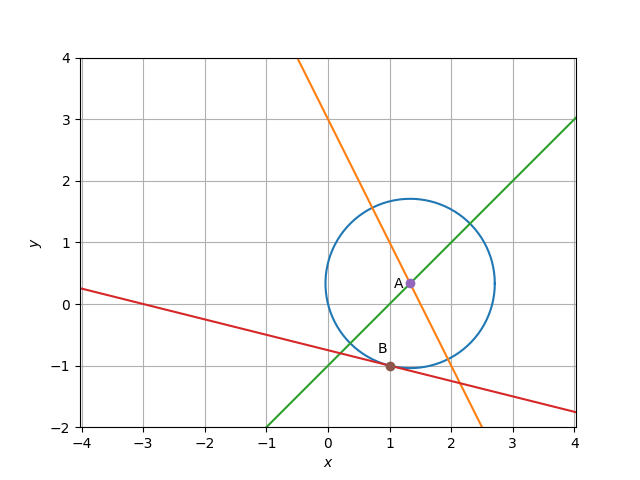
\includegraphics[width=\textwidth]{preambule/matrix-2.png}\\
using the code above figure can be obtained and  tangent equation can be computed-\\
\begin{lstlisting}[language=Python]
import numpy as np 
import matplotlib.pyplot as plt
a=np.array([2,1])
b=np.array([1,-1])

N1=np.vstack((a,b))
p1=np.array([3,1])
A=np.matmul(np.linalg.inv(N1),p1)

B=np.array([1,-1])
n=np.matmul(np.array([[0,-1],[1,0]]),B-A)
r=np.linalg.norm(B-A)
len=100

print(n)


x1=np.zeros((2,len))
x2=np.zeros((2,len))
x3=np.zeros((2,len))
x4=np.zeros((2,len))
lam1=np.linspace(0,2*np.pi,len)
lam2=np.linspace(-10,10,len)


for i in range(len):
	temp1= np.array([A[0]+r*np.cos(lam1[i]),A[1]+r*np.sin(lam1[i])])
	x1[:,i]=temp1.T
for i in range(len):
	temp1= np.array([lam2[i],3-2*(lam2[i])])
	x2[:,i]=temp1.T
for i in range(len):
	temp1= np.array([lam2[i],lam2[i]-1])
	x3[:,i]=temp1.T	
for i in range(len):
	temp1=B+lam2[i]*n
	x4[:,i]=temp1.T
plt.plot(x1[0,:],x1[1,:])
plt.axis('equal')
plt.plot(x2[0,:],x2[1,:])
plt.axis('equal')
plt.plot(x3[0,:],x3[1,:])
plt.axis('equal')
plt.plot(x4[0,:],x4[1,:])
plt.axis('equal')
plt.plot(A[0],A[1],'o')
plt.text(A[0]*(1-0.2),A[1]*(1-0.2),'A')
plt.plot(B[0],B[1],'o')
plt.text(B[0]*(1-0.2),B[1]*(1-0.2),'B')
plt.xlabel('$x$')
plt.ylabel('$y$')
plt.xlim(-3,5)
plt.ylim(-3,5)
	
	
plt.grid()
plt.show()
	

\end{lstlisting}

\end{document}












 
